% Chapter 4

\chapter{Layout} % Write in your own chapter title
\label{Chapter4} 
\lhead{\emph{Layout}}

In Fig. \ref{fig:layout} si può ammirare il layout finale del Full Adder TSPC.

\begin{figure}[hbt!]
	\centering
	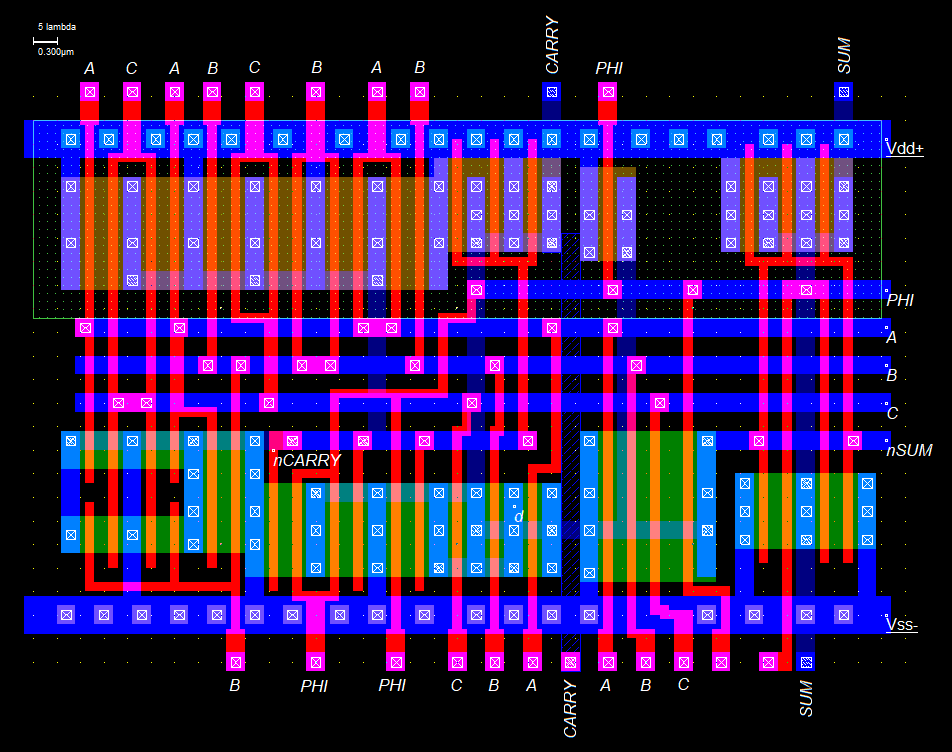
\includegraphics[width=1\textwidth]{figure/Msk_FullDesign.png}
	\caption{Layout finale.}
	\label{fig:layout}
\end{figure}

Vediamo quali sono stati i passi che hanno portato alla sua realizzazione.

\section{Disegno dei singoli stadi}
\label{sec:sec_disegnoStadi}

Un possibile metodo di lavoro prevede di ottenere il circuito finale in maniera progressiva, realizzando e validando un singolo stadio alla volta, mediante simulazioni \textit{post-layout}. Il circuito finale è ottenuto dall'unione dei vari pezzi ed è a sua volta validato da una simulazione dello stesso tipo che, se soddisfacente, sancisce il raggiungimento degli obiettivi prefissati. 

Analizziamo quindi i disegni delle singole parti di circuito riportando alcuni screen tratti da \textit{Microwind} e i cui colori hanno i seguenti significati:

\begin{itemize}
	\item lo sfondo nero rappresenta il substrato di tipo \textit{p};
	\item le aree verdi sono diffusioni di tipo \textit{n};
	\item le aree verdi a puntini sono diffusioni di tipo \textit{n-well};
	\item le aree rosse costituiscono piste di polisilicio;
	\item le aree blu sono metalizzazioni di tipo \textit{metal 1}; 
	\item i quadrati con la croce all'interno indicano la presenza di un contatto tra livelli differenti.
\end{itemize}

\subsection{Stadio \textit{1} - Generazione di !CARRY}

In fig. \ref{fig:NMOSePMOSnotCarry} si può osservare la realizzazione della parte \textit{n} (a sinistra) e della parte \textit{p} (a destra) dello stadio \textit{1} dedicato alla generazione del segnale \textit{!CARRY}, indicato nel layout con la label \textit{notCarry}. I MOS più larghi sono disegnati "ripiegati" su se stessi in modo da mantenere le dimensioni di canale desiderate pur potendo riorganizzare la disposizione delle diffusioni per meglio adattarsi alla forma generale che si vuole far assumere al circuito. 

Per ciascuno dei due circuiti viene estratta la netlist che, tramite \textit{LTspice}, permette di validare il disegno tenendo conto di tutti i parametri presenti nel modello della tecnologia utilizzata, incluse le capacità parassite.

\begin{figure}[hbt!]
	\centering
	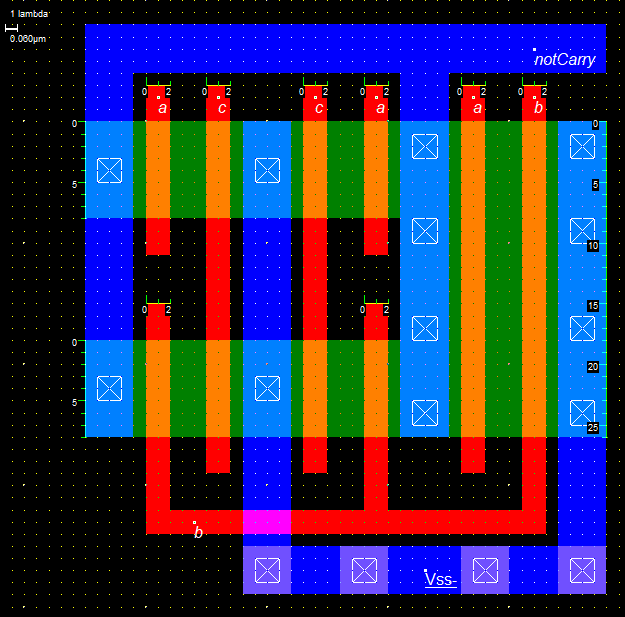
\includegraphics[width=0.4\textwidth]{figure/Msk_NMOS_notCarry_V2.png}\hfil
	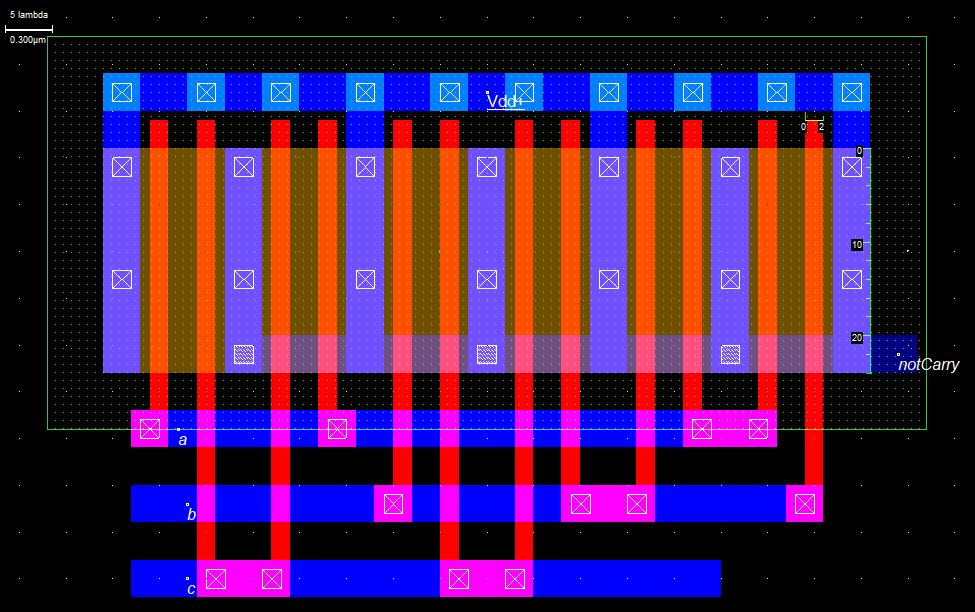
\includegraphics[width=0.4\textwidth]{figure/Msk_PMOS_notCarry_V2.png}
	\caption{Parte \textit{n} (a sinistra) e parte \textit{p} (a destra) dello stadio 1.}
	\label{fig:NMOSePMOSnotCarry}
\end{figure} 

Le due parti collegate costituiscono il disegno complessivo dello stadio \textit{1}, riportato in fig. \ref{fig:notCarry}. Da tale figura si può notare la scelta di adottare un approccio \textit{standard cell} per la disposizione delle piste di alimentazione e di segnale, come d'altronde viene suggerito nelle specifiche di progetto. In alto e in basso sono quindi presenti due piste orizzontali di \textit{Metal 1} collegate rispettivamente all'alimentazione positiva e negativa. I segnali \textit{A}, \textit{B}, \textit{C} e \textit{notCarry} sono forniti e prelevati in verticale, tramite piste di polisilicio per i primi tre e una pista di \textit{Metal 2} per l'ultimo. Tutti e quattro, assieme a \textit{phi}, sono poi trasportati nel resto del circuito da alcune piste di \textit{Metal 1}, orizzontali, poste tra le parti \textit{n} e le parti \textit{p} di ogni stadio.

\begin{figure}[hbt!]
	\centering
	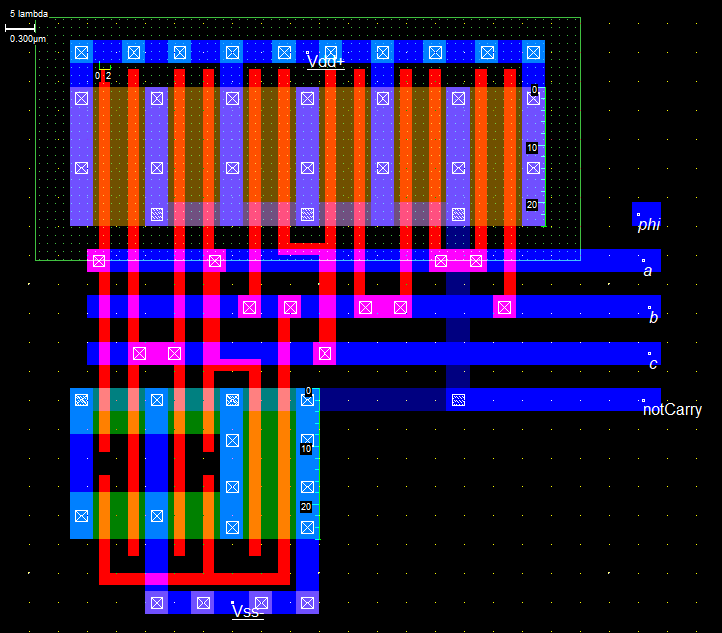
\includegraphics[width=0.5\textwidth]{figure/Msk_NotCarry_V2.png}
	\caption{Disegno dello stadio \textit{1} dedicato alla generazione di \textit{notCarry}.}
	\label{fig:notCarry}
\end{figure} 

Anche di questo circuito si effettua una simulazione \textit{post-layout} prima di procedere allo stadio successivo.

\subsection{Stadio \textit{2.1} - Generazione di !SUM}

In figura \ref{fig:NMOSnotSum} è riportato il disegno della parte \textit{n} dello stadio \textit{2.1} dedicato alla generazione del segnale \textit{!SUM}, etichettato come \textit{notSum}. Una particolarità di questa parte riguarda la realizzazione dei MOS in serie, ottenuta tramite l'affiancamento di diverse piste di polisilicio pilotate dai segnali d'ingresso; questa tecnica permette di risparmiare spazio evitando di inserire metalizzazioni per i gate dei MOS intermedi tra il nodo di uscita \textit{notSum} e il nodo comune ai due rami che compongono questa parte di circuito: non è infatti necessario prelevare tali segnali.

\begin{figure}[hbt!]
	\centering
	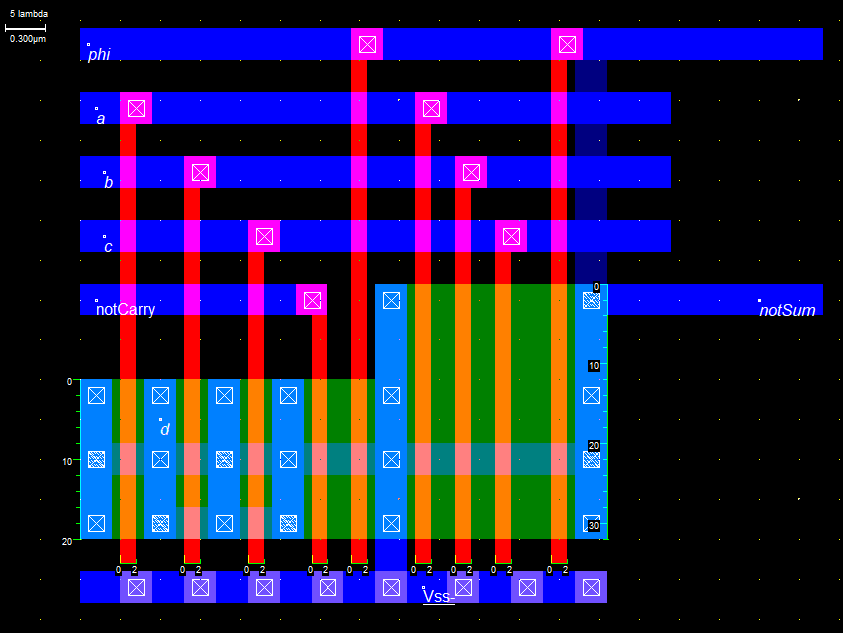
\includegraphics[width=0.5\textwidth]{figure/Msk_NMOS_NotSum.png}
	\caption{Parte \textit{n} dello stadio \textit{2.1} dedicato alla generazione di \textit{notSum}.}
	\label{fig:NMOSnotSum}
\end{figure} 

La parte \textit{p} di questo stadio è costituita da un semplice pMOS per cui se ne omette la rappresentazione completa. Considerazioni circa la tipologia di progetto \textit{standard cell} e la procedura di validazione sono analoghe a quelle esposte per lo stadio \textit{1}.

\subsection{Stadi finali \textit{2.2} e \textit{3} - Generazione di CARRY e SUM}

Gli stadi finali \textit{2.2} e \textit{3} hanno la stessa identica struttura, per cui per brevità si riporta in fig. \ref{fig:sum} il disegno del solo stadio \textit{3}, dedicato alla generazione del segnale d'uscita \textit{SUM}.

\begin{figure}[hbt!]
	\centering
	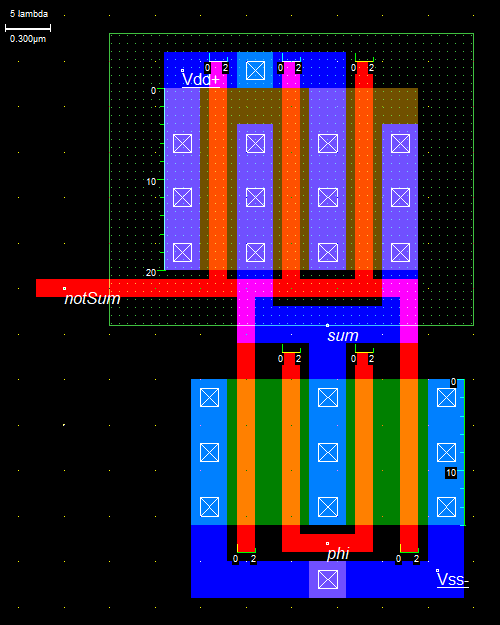
\includegraphics[width=0.5\textwidth]{figure/Msk_SumInveter.png}
	\caption{Disegno dello stadio \textit{3} dedicato alla generazione di \textit{SUM}.}
	\label{fig:sum}
\end{figure} 

Le tecniche utilizzate per il layout di questi stadi sono le stesse già presentate nei paragrafi precedenti. Terminata la sua validazione, si può procedere a comporre il circuito finale.

\section{Full design}
\label{sec:sec_fullDesign}

Il circuito finale, rappresentato in fig. \ref{fig:layout}, è il risultato della composizione dei singoli stadi presentati finora. Essi sono affiancati in modo da ottenere una struttura tanto più compatta possibile pur mantenendo la topologia delle varie parti. Ciò significa avvicinare le varie piste e/o diffusioni in modo da minimizzare gli spazi vuoti pur rispettando le regole di progettazione ovvero le distanze minime necessarie. 

Il risultato è un circuito molto ordinato e di dimensioni $11.04 \mu m \times 6.54 \mu m$ (ovvero, in \textit{lambda}, 184 x 109), con i segnali di ingresso/uscita prelevati e forniti in verticale e quelli di alimentazione applicati in orizzontale.

L'ultimo passo consiste nel compiere un'ultima validazione del circuito finale. Se ne esporta quindi la netlist che viene simulata tramite \textit{LTspice}. Il risultato della simulazione si osserva in fig. \ref{fig:simulazioneFinale}. Come si può notare a fronte di ogni combinazione degli ingressi \textit{A}, \textit{B}, \textit{C}, i segnali \textit{SUM} e \textit{CARRY} assumono il livello di tensione corretto entro le tempistiche richieste.  

\begin{figure}[hbt!]
	\centering
	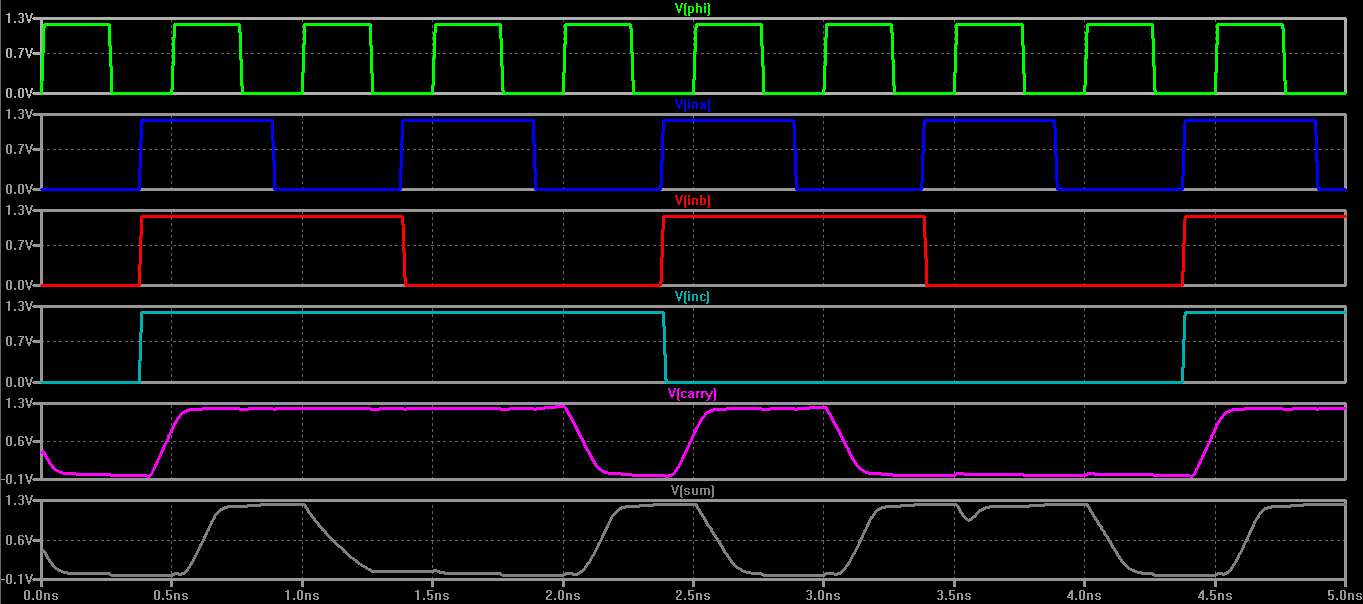
\includegraphics[width=1.5\textwidth, angle=90]{figure/Sim_FullDesign_PostLayout.PNG}
	\caption{Simulazione post-layout dello stadio finale.}
	\label{fig:simulazioneFinale}
\end{figure}

Da questa simulazione è anche possibile calcolare la potenza media dissipata dal circuito in esame, che risulta pari a $315\mu W$.






